\documentclass[a4paper,11pt]{article}
%\usepackage[T1]{fontenc}

%\setlength{\textwidth}{20cm}
%\setlength{\marginparwidth}{0cm}
%\setlength{\voffset}{0cm}
\usepackage[utf8]{inputenc}
\usepackage[francais]{babel}
\usepackage{amsmath}
\usepackage{graphicx}
\usepackage{float}
\usepackage{slashbox}
%\special{papersize=210mm,297mm}

\title{{\Huge Electronique numérique}\\Logique séquentielle}
%\title{TD1}

\begin{document}
\maketitle

{\it Tous les exercices ne seront pas résolus en TE}

\section{Découverte de la bascule D}
Le symbole de la bascule D, ainsi que sa table de vérité sont rappelés ici.\\

\begin{figure}[!h]
\begin{center}
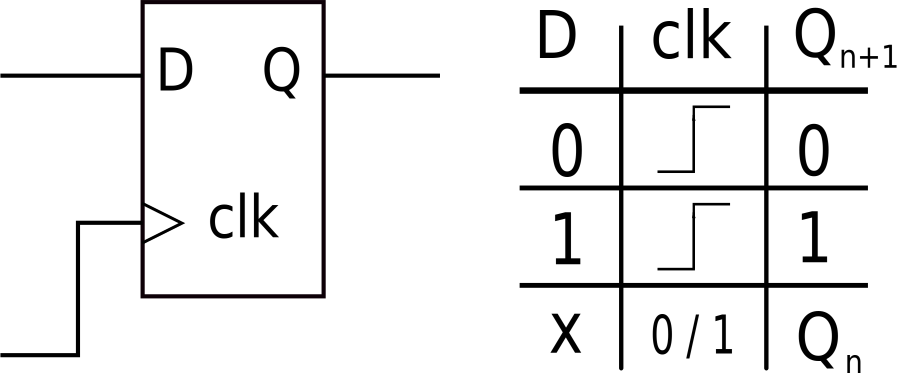
\includegraphics[scale=0.2]{./figures/d-ff-infos.jpg}
\end{center}
\end{figure}

La bascule D a pour fonction de recopier l'entrée D sur sa sortie Q, lors d'un court temps d'échantillonnage : il s'agit généralement du front montant de l'horloge. Cette horloge est supposée périodique. Pour que l'échantillonnage se passe correctement, le signal d'entrée doit respecter deux contraintes : il doit être parfaitement stable {\it avant} et {\it après} le front montant. Ces instants s'appellent temps de {\it setup} et temps de {\it hold}. La donnée est électriquement recopiée après un instant également très court appelé ``clock to Q''. Tous ces temps sont très inférieurs à la période d'horloge. {\bf La bascule D permet ainsi de travailler sur un signal stable, pendant toute une période} : le temps est désormais {\bf discrétisé}. Il n'y a plus à se soucier des temps de propagation caractéristiques -- et parfois fluctuants-- des différentes portes logiques réalisant les calculs ! Il suffit d'attendre une période d'horloge suffisamment longue pour observer un résultat combinatoire correct, échantillonné dans une bascule. L'écoulement du temps ne se fait que par 'quantum' de temps : celui des 'tops' (ou 'ticks') de cette horloge périodique. Il est même possible d'abstraire le fonctionnement du circuit encore plus en supposant que seuls ces instants d'échantillonnage sont significatifs et que les calculs s'effectuent instantanément sur ces 'tops' (on parle de calcul en ``temps zéro''), et que rien ne se passe entre ces 'tops' ! Mais cela reste 'une vue de l'esprit'.\\

Compléter le chronogramme suivant où un signal $S_1$ sur 4 bits, extérieur au système et asynchrone, est fourni comme entrée (sous sa forme entière).

\begin{figure}[!h]
\begin{center}
\includegraphics[scale=0.4]{./figures/dff-1.png}
\end{center}
\end{figure}


On précise ici que :
\begin{itemize}
\item nous ne tenons pas compte de la notion de temps de {\it setup} et temps de {\it hold}, ni du temps $t_{clk-2-Q}$
\item les zones de transistion des 4 bits se présentent ici comme des 'X'.
\item pour les signaux internes au système, on ne représentera pas ces transitions, supposées idéales : seuls des rectangles suffiront.
\item on suppose que les sorties Q sont initialisées à 0.
\end{itemize}

{\bf solution}

\begin{figure}[!h]
\begin{center}
\includegraphics[scale=0.4]{./figures/dff-1-CORR-1.png}
\end{center}
\end{figure}

Les plus observateurs noteront que le signal S5 possède deux valeurs $16$ et $21$ qui ne peuvent pas être
encodées sur 4 bits (il en faut 5). Toutefois, dans cet exercice, rien ne stipule que tous les signaux
doivent forcément être encodés sur 4 bits. Malgré tout, si on impose cette contrainte de 4 bits sur tous les
signaux, ces deux valeurs seront tronquées : $16$ sera tronqué à $0$ et $21$ sera tronqué à $5$. Dans les 2 cas, le MSB à 1 en position 5 est perdu.

Une autre question récurrente sur cet exercice est la suivante : on a expliqué que l'échantillonnaghe de S1 ne peut pas bien se passer sur la valeur incertaine entre 8 et 5.
Le déclanchement de la recopie, par la bascule, sur front montant intervient sur un signal instable et dont la valeur ne peut être connue avec certitude.
Pourtant, la solution proposée à l'exercice conduit à dessiner de tels cas semblables, partout dans le tableau : les transitions entre les valeurs sont inscrites sur le front lui-même, ce qui
a de quoi perturber...En réalité, la bascule D possède deux fonctions : vis-à-vis d'un signal externe (comme S1), non-synchronisé sur l'horloge, la bascule permettra de filter le signal, en ne conservant que
les valeurs se prêtant à un échantillonnage correct (respect des temps de setup et de hold). Ensuite, en interne, la bascule D, réalise la simple recopie de l'entrée, décallée d'un cycle
d'horloge. Une autre manière de voir les choses, et qui permet d'éviter de considérer 2 fonctions distinctes à la bascule, est d'insérer des temps $\delta t_i$ infinitésimal entre l'instant précis
du front montant et l'apparition de la valeur sur $Q_i$. Physiquement, ces temps existent (clk-to-Q). Toutefois, il est préférable de ne plus les considérer (on les fait tendre vers 0) : cela
 permet de simplifier les raisonnements, en retombant dans le monde des suites numériques, plutôt que de conserver ces grandeurs temporelles physiques, par ailleurs compliquées à dessiner !
 Il s'agit d'une abstraction, qui fonctionne très bien dans le cas des circuits numériques synchrones. Pour rappel, une abstraction cherche à gommer les détails inutiles (ici le temps physique), tout en conservant les propriétés essentielles (ici la recopie) de l'objet considéré (la bascule)


%===========================================================================
\newpage
\section{Du circuit au chronogramme}

Soit le circuit logique suivant.

\begin{figure}[!h]
\begin{center}
\includegraphics[scale=0.3]{./figures/fsm-ex1.png}
\end{center}
\end{figure}

Sachant que la bascule D est initialisée à 0, trouver le chronogramme de la sortie $out$ correspondante, lorsque les valeurs d'entrée sont (respectivement, à chaque coup d'horloge) :

\begin{verbatim}
e1 : 0 1 0 1 1 0 1
e2 : 1 1 1 0 1 0 0
\end{verbatim}

{\bf Corrections}

On commence par le cycle 1 : on connaît la valeur de $e1=0$ à ce cycle, ainsi que la valeur $Q=0$ (comme indiqué dans l'énoncé).
On en déduit : la sortie du AND vaut $0$. D'où, connaissant $e2=1$, on
trouve la sortie du OR égale à $1$.Cette sortie du OR est également l'entrée D de la bascule.
Enfin, pour ce premier cycle, on détermine la sortie OUT, qui vaut $0$. On peut donc passer
au cycle 2 : pour cela il faut commencer par dépercuter la valeur précédente ($1$) sur D vers la sortie Q courante de la bascule. Ainsi, Q, au cycle 2, vaut $1$.
A partir de là, on peut continuer à propager les calculs, de proche en proche.
Un calcul combinatoire impose de rester dans l'instant courant, alors qu'un élément séquentiel (bascule D), impose de se déplacer dans le temps, discrétisé.
On trouve le chronogramme complet :

\begin{figure}
\begin{center}
      \begin{tabular}{|c||c|c|c|c|c|c|c|}
          \hline
          cycle  & 1 & 2 & 3 & 4 & 5 & 6 & 7 \\ \hline \hline
          e1     & 0 & 1 & 0 & 1 & 1 & 0 & 1   \\ \hline
          e2     & 1 & 1 & 1 & 0 & 1 & 0 & 0  \\ \hline
          and    & 0 & 1 & 0 & 1 & 1 & 0 & 0   \\ \hline
          or     & 1 & 1 & 1 & 1 & 1 & 0 & 0   \\ \hline
          D      & 1 & 1 & 1 & 1 & 1 & 0 & 0   \\ \hline
          Q      & 0 & 1 & 1 & 1 & 1 & 1 & 0   \\ \hline
          Out    & 0 & 1 & 1 & 0 & 1 & 0 & 0   \\ \hline
      \end{tabular}
\end{center}
\end{figure}
%===========================================================================
\newpage
\section{Du chronogramme au circuit}
Nous proposons ici un exercice plus rare, uniquement par jeu : il s'agit de retrouver le circuit qui a généré les chronogrammes suivants.
Il y a probablement plusieurs solutions ! Soyez perspicaces ! Les signaux $e_i$ représentent des entrées, les signaux $s_i$ des sorties, et les signaux $n_i$ des signaux internes.

\begin{verbatim}
      e1 : 0 0 1 1 0 0 0 0 1 1 0 0 1 0 0 0 0
      e2 : 0 0 0 0 1 0 0 1 0 1 1 0 1 1 0 0 0
      n1 : 0 0 1 1 1 0 0 1 1 1 1 0 1 1 0 0 0
      s1 : 0 0 1 0 0 0 0 1 0 0 0 0 1 0 0 0 0
      s2 : 1 1 0 1 1 1 1 0 1 1 1 1 0 1 1 1 1
      s3 : ? 1 1 0 1 1 1 1 0 1 1 1 1 0 1 1 1
\end{verbatim}


{\bf solution :}

On voit que :
\begin{itemize}
\item $n1$ est le OU entre $e1$ et $e2$
\item $s1$ marque le debut de la sequence des 1 de $n1$ ( $\rightarrow n1_t.\overline{n1_{t-1}}$)
\item $s2_t$ est l'inverse de $s1_t$
\item $s3$ est égal au signal $s2$, décallé d'un cycle : $s3_t=s2_{t-1}$
\end{itemize}

Un circuit possible est alors :
\begin{figure}[!h]
\begin{center}
\includegraphics[scale=0.3]{./figures/exo5-circuit.png}
\end{center}
\end{figure}


% \section{Du circuit au diagramme à bulles}
% On reprend ici l'exercice 2. En supposant que la bascule se trouve dans l'état 0 au démarrage du circuit, décrire le diagramme à bulle du système.\\
%
% {\bf solution : }
%
% Le circuit ne possède qu'une seule bascule D donc un seul bit d'état, ce qui va beaucoup nous aider. On écrit la table de vérité de la fonction de transition $f_{trans}(e_1,e_2,Q)$ :
%
% \begin{table}[H]
% \begin{center}
%     \begin{tabular}{|c|c|c||c||c|}
%         \hline
%         e1 & e2 & Q & D & ligne \\ \hline \hline
%         0  & 0  & 0 & 0 & 0 \\
%         0  & 0  & 1 & 0 & 1 \\
%         0  & 1  & 0 & 1 & 2 \\
%         0  & 1  & 1 & 1 & 3 \\
%         1  & 0  & 0 & 0 & 4 \\
%         1  & 0  & 1 & 1 & 5 \\
%         1  & 1  & 0 & 1 & 6 \\
%         1  & 1  & 1 & 1 & 7 \\
%         \hline
%     \end{tabular}
% \end{center}
% \end{table}
%
% Appelons E cette variable d'état. L'état courant de E est matérialisé par Q et sont état futur par D. Comment évolue cette variable au cours du temps ? On peut dessiner le diagramme à bulle suivant (ou diagramme d'état), et faire donc apparaître 4 conditions booléennes possibles, appelées $k_1,k_2,k_3,k_4$, relatives aux transitions. \\
%
% \begin{figure}[H]
% \begin{center}
% \includegraphics[scale=0.2]{./figures/exo5.png}
% \end{center}
% \end{figure}
%
% Trouvons alors ces $k_1,k_2,k_3,k_4$ :\\
%
% \begin{itemize}
% \item E passe de 0 à 0 sur les lignes 0 et 4 d'où la condition $k_1=\overline{e_2}$
% \item E passe de 0 à 1 sur les lignes 2 et 6 d'où la condition $k_2=e_2$ (soit encore $k_2=\overline{k_1}$).
% \item E passe de 1 à 1 sur les lignes 3, 5 et 7 d'où la condition $k_3=e_1+e_2$
% \item E passe de 1 à 0 sur les lignes 1, d'où la condition $k_4=\overline{e_1}.\overline{e_2}$ (soit encore $k_4=\overline{k_3}$).
% \end{itemize}

\section{Suite de Fibonacci en circuit}
La suite de Fibonacci est bien connue : $u_{n+2}=u_{n+1}+u_{n}$, où $u_{1}=1$ et $u_0=0$.
Elle date de 1202 et décrit la croissance d'une population de lapins, à partir d'un seul couple.
Pour la petite histoire, cette suite a par ailleurs un lien étonnant avec le nombre d'or $\phi=\frac{1+\sqrt{5}}{2} \approx 1.628$.
En effet, Euler a démontré que pour un $n$ donné (un "step"), on a :
$$u_n=\frac{1}{\sqrt{5}}(\phi^n - \phi'^n) \textrm{ , où } \phi' = - \frac{1}{\phi}$$

\begin{enumerate}
  \item Dessiner le circuit numérique émettant la suite de Fibonacci. Un changement d'indice simple, au préalable, est conseillé.
  \item Chaque bascule D possède un reset actif haut, et un set actif bas. Compléter le schéma précédent, de manière à initialiser correctement les bascules. On dispose d'un bouton poussoir
  d'initialisation qui fournit un signal de {\it reset} actif {\it haut} : lorsqu'on appuie sur ce bouton pour initialiser le circuit, ce signal vaut '1'.
\end{enumerate}

\boxed{Solution}

\begin{enumerate}

  \item On fait le changement d'indice suggéré : $u_n=u_{n-1}+u_{n-2}$. Le décalage temporel correspond à une bascule D. On a donc le schéma \ref{fibo1}.
  On a omis le signal d'horloge, supposé présent de manière implicite.

  \begin{figure}[H]
    \begin{center}
      \includegraphics[scale=0.3]{./figures/fibo1.png}
      \label{fibo1}
    \end{center}

 \end{figure}

  \item L'initialisation se fait comme présenté sur le schéma \ref{fibo2}
  \begin{figure}[H]
    \begin{center}
      \includegraphics[scale=0.3]{./figures/fibo2.png}
      \label{fibo2}
    \end{center}

  \end{figure}


\end{enumerate}

\end{document}
